\documentclass[a4paper,12pt]{article}
\usepackage[ukrainian,english]{babel}
\usepackage{ucs}
\usepackage[utf8]{inputenc}
\usepackage[T2A]{fontenc}
\usepackage{amsmath}
\usepackage{amsfonts}
\usepackage[final]{graphicx}
\usepackage{subfigure}
\usepackage{wrapfig}
\usepackage{multirow}
\usepackage{flafter}
\usepackage{lscape}
\usepackage{caption}
\usepackage{float}
\usepackage[caption = false]{subfig}
\usepackage{rotating}
\usepackage{booktabs}
\newcommand\tab[1][1cm]{\hspace*{#1}}
\usepackage[left=20mm, top=20mm, right=10mm, bottom=20mm, nohead, nofoot]{geometry}
\usepackage{blindtext}
\begin{document}
\begin{titlepage}
\begin{center}
\large НАЦІОНАЛЬНИЙ ТЕХНІЧНИЙ УНІВЕРСИТЕТ УКРАЇНИ «КИЇВСЬКИЙ ПОЛІТЕХНІЧНИЙ ІНСТИТУТ» ФІЗИКО-ТЕХНІЧНИЙ ІНСТИТУТ	
\newline\newline\newline\newline\newline\newline\newline\newline\newline
\LARGE{ЛАБОРАТОРНА РОБОТА З ФІЗИКИ № 3.1\\ $\>\>\>\>\>\>\>$ВИВЧЕННЯ ФІЗИЧНОГО МАЯТНИКА}
\newline\newline\newline\newline\newline\newline\newline\newline\newline
\end{center}
\flushright 
Виконала:\\
студент групи  ФІ-12\\
Бекешева Анастасія \\
Прийняв:\\
Долгошей В.Б.

\end{titlepage}
\newpage
\section{Обробка результатів експерименту}
% Please add the following required packages to your document preamble:
% \usepackage{multirow}
\begin{table}[htp]\centering
\caption{Фізичний маятник}
\begin{tabular}{|c|c|c|c|c|c|c|c|c|c|c|c|c|}
\hline
$N$                 & $L$                    & $t$   & $T$  & $\langle T\rangle$     & $g$                   & $\langle g\rangle$    & $\Delta g$           & $\varepsilon(g)$       & $L_{\textrm{теор}}$    & $\Delta L$             & $\varepsilon(L)$       & $\varepsilon(L)_{\textrm{сер}}$ \\ \hline
\multirow{9}{*}{10} & \multirow{3}{*}{0.397} & 12.56 & 1.26 & \multirow{3}{*}{1.287} & \multirow{3}{*}{9.467}  & \multirow{9}{*}{10.335} & \multirow{9}{*}{0.525} & \multirow{9}{*}{5$\%$} & \multirow{3}{*}{0.38}  & \multirow{3}{*}{0.017} & \multirow{3}{*}{4$\%$} & \multirow{9}{*}{5$\%$}          \\ \cline{3-4}
                    &                        & 13.01 & 1.3  &                        &                       &                       &                      &                        &                        &                        &                        &                                 \\ \cline{3-4}
                    &                        & 13.02 & 1.3  &                        &                       &                       &                      &                        &                        &                        &                        &                                 \\ \cline{2-6} \cline{10-12}
                    & \multirow{3}{*}{0.387} & 12.11 & 1.21 & \multirow{3}{*}{1.213} & \multirow{3}{*}{10.378} &                       &                      &                        & \multirow{3}{*}{0.365} & \multirow{3}{*}{0.022} & \multirow{3}{*}{6$\%$} &                                 \\ \cline{3-4}
                    &                        & 12.24 & 1.22 &                        &                       &                       &                      &                        &                        &                        &                        &                                 \\ \cline{3-4}
                    &                        & 12.06 & 1.21 &                        &                       &                       &                      &                        &                        &                        &                        &                                 \\ \cline{2-6} \cline{10-12}
                    & \multirow{3}{*}{0.361} & 11.26 & 1.13 & \multirow{3}{*}{1.13}  & \multirow{3}{*}{11.116} &                       &                      &                        & \multirow{3}{*}{0.38}  & \multirow{3}{*}{0.019} & \multirow{3}{*}{5$\%$} &                                 \\ \cline{3-4}
                    &                        & 11.26 & 1.13 &                        &                       &                       &                      &                        &                        &                        &                        &                                 \\ \cline{3-4}
                    &                        & 11.26 & 1.13 &                        &                       &                       &                      &                        &                        &                        &                        &                                 \\ \hline
\end{tabular}
\caption{Прямий та оборотний маятники}
\begin{tabular}{|c|c|c|c|c|c|c|c|c|c|c|c|c|}
\hline
$N$                 & $S_1$                  & $S_2$                  & $t_1$ & $t_2$ & $T_1$ & $T_2$ & $\langle T_1\rangle$  & $\langle T_2\rangle$  & $T_0$                       & $g$                    & $\Delta g$             & $\varepsilon(g)$           \\ \hline
\multirow{9}{*}{10} & \multirow{3}{*}{0.21}  & \multirow{3}{*}{0.17}  & 12.78 & 12.5  & 1.28  & 1.25  & \multirow{3}{*}{1.28} & \multirow{3}{*}{1.25} & \multirow{9}{*}{1.41627446} & \multirow{9}{*}{10.59} & \multirow{9}{*}{0.782} & \multirow{9}{*}{7.394$\%$} \\ \cline{4-7}
                    &                        &                        & 12.73 & 12.47 & 1.27  & 1.25  &                       &                       &                             &                        &                        &                            \\ \cline{4-7}
                    &                        &                        & 12.96 & 12.46 & 1.30  & 1.25  &                       &                       &                             &                        &                        &                            \\ \cline{2-9}
                    & \multirow{3}{*}{0.12}  & \multirow{3}{*}{0.245} & 12.60 & 11.01 & 1.26  & 1.10  & \multirow{3}{*}{1.25} & \multirow{3}{*}{1.1}  &                             &                        &                        &                            \\ \cline{4-7}
                    &                        &                        & 12.52 & 11.01 & 1.25  & 1.10  &                       &                       &                             &                        &                        &                            \\ \cline{4-7}
                    &                        &                        & 12.52 & 11.01 & 1.25  & 1.10  &                       &                       &                             &                        &                        &                            \\ \cline{2-9}
                    & \multirow{3}{*}{0.105} & \multirow{3}{*}{0.275} & 12.35 & 12.56 & 1.24  & 1.26  & \multirow{3}{*}{1.24} & \multirow{3}{*}{1.26} &                             &                        &                        &                            \\ \cline{4-7}
                    &                        &                        & 12.36 & 12.55 & 1.24  & 1.26  &                       &                       &                             &                        &                        &                            \\ \cline{4-7}
                    &                        &                        & 12.34 & 12.55 & 1.23  & 1.26  &                       &                       &                             &                        &                        &                            \\ \hline
\end{tabular}
% Please add the following required packages to your document preamble:
% \usepackage{multirow}
\caption{Залежність $L$ від $T^2$}
\begin{tabular}{|cccccccc|}
\hline
\multicolumn{1}{|c|}{$T^2$} & \multicolumn{1}{c|}{$L$}   & \multicolumn{1}{c|}{$g_1$}                 & \multicolumn{1}{c|}{$g_2$}                  & \multicolumn{1}{c|}{$g_3$}                  & \multicolumn{1}{c|}{$\langle g\rangle$}     & \multicolumn{1}{c|}{$\Delta g$}            & $\varepsilon g$           \\ \hline
\multicolumn{1}{|c|}{1.66}  & \multicolumn{1}{c|}{0.397} & \multicolumn{1}{c|}{\multirow{3}{*}{9.44}} & \multicolumn{1}{c|}{\multirow{3}{*}{10.39}} & \multicolumn{1}{c|}{\multirow{3}{*}{11.22}} & \multicolumn{1}{c|}{\multirow{3}{*}{10.35}} & \multicolumn{1}{c|}{\multirow{3}{*}{0.54}} & \multirow{3}{*}{5.24$\%$} \\ \cline{1-2}
\multicolumn{1}{|c|}{1.47}  & \multicolumn{1}{c|}{0.387} & \multicolumn{1}{c|}{}                      & \multicolumn{1}{c|}{}                       & \multicolumn{1}{c|}{}                       & \multicolumn{1}{c|}{}                       & \multicolumn{1}{c|}{}                      &                           \\ \cline{1-2}
\multicolumn{1}{|c|}{1.27}  & \multicolumn{1}{c|}{0.361} & \multicolumn{1}{c|}{}                      & \multicolumn{1}{c|}{}                       & \multicolumn{1}{c|}{}                       & \multicolumn{1}{c|}{}                       & \multicolumn{1}{c|}{}                      &                           \\ \hline
                            &                            &                                            &                                             &                                             &                                             &                                            &                           \\ \hline
\multicolumn{1}{|c|}{$T^2$} & \multicolumn{1}{c|}{$L$}   & \multicolumn{1}{c|}{$g_1$}                 & \multicolumn{1}{c|}{$g_2$}                  & \multicolumn{1}{c|}{$g_3$}                  & \multicolumn{1}{c|}{$\langle g\rangle$}     & \multicolumn{1}{c|}{$\Delta g$}            & $\varepsilon g$           \\ \hline
\multicolumn{1}{|c|}{1.64}  & \multicolumn{1}{c|}{0.397} & \multicolumn{1}{c|}{\multirow{3}{*}{9.56}} & \multicolumn{1}{c|}{\multirow{3}{*}{9.73}}  & \multicolumn{1}{c|}{\multirow{3}{*}{9.31}}  & \multicolumn{1}{c|}{\multirow{3}{*}{9.53}}  & \multicolumn{1}{c|}{\multirow{3}{*}{0.28}} & \multirow{3}{*}{2.89$\%$} \\ \cline{1-2}
\multicolumn{1}{|c|}{1.57}  & \multicolumn{1}{c|}{0.387} & \multicolumn{1}{c|}{}                      & \multicolumn{1}{c|}{}                       & \multicolumn{1}{c|}{}                       & \multicolumn{1}{c|}{}                       & \multicolumn{1}{c|}{}                      &                           \\ \cline{1-2}
\multicolumn{1}{|c|}{1.53}  & \multicolumn{1}{c|}{0.361} & \multicolumn{1}{c|}{}                      & \multicolumn{1}{c|}{}                       & \multicolumn{1}{c|}{}                       & \multicolumn{1}{c|}{}                       & \multicolumn{1}{c|}{}                      &                           \\ \hline
\end{tabular}
\end{table}\newpage
\section{Графіки}
\begin{center}
	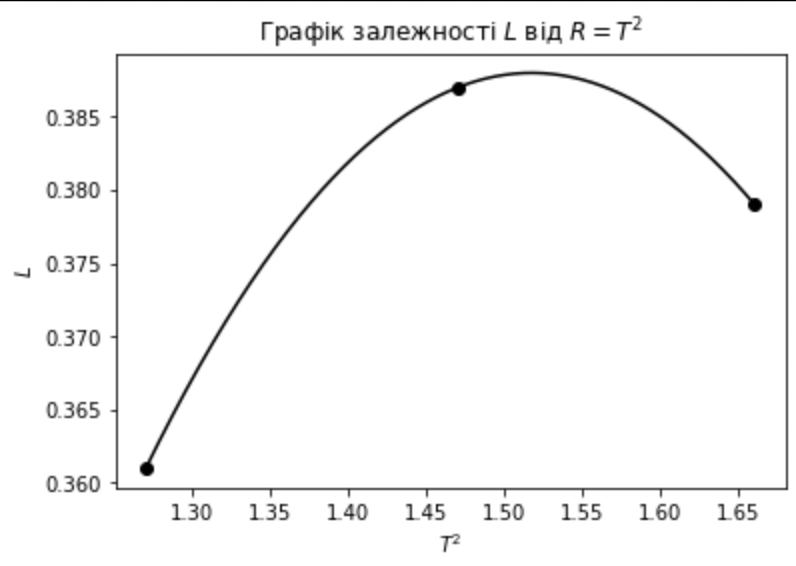
\includegraphics[width=10cm]{graph7}
	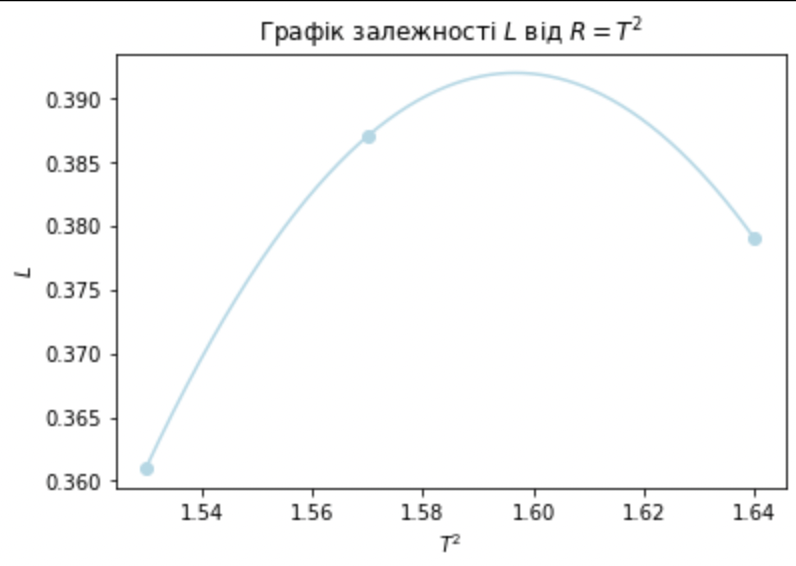
\includegraphics[width=10cm]{graph8}
\end{center}
\newpage\section{Висновок}
За результатами обробки дослідних даних отримані прискорення вільного падіння для кожного з періодів (фізичного та приведеного), визначених у ході експерименту, а також прискорення вільного падіння з урахуванням різниці  періодів.
Результатом експерименту є таке отримане за допомогою оборотного маятника значення прискорення вільного падіння: $g=9.5\pm0.78$ м/с$^2$ 
Похибка експерименту склала 7,39$\%$. Похибки виникли за впливу таких факторів як не точне зведення періодів, інструментальні похибки та похибки вимірювання, недостатня точність визначення положення центра мас, не врахування дії сил тертя (внаслідок стертості призм).





























\end{document}